\documentclass{IEEEtran}

\usepackage{cite}
\usepackage{amsmath}
\usepackage{amssymb}
\usepackage{url}
\usepackage{graphicx}
\usepackage{booktabs}
\usepackage{microtype}
\usepackage[table]{xcolor}
\usepackage{tikz}
\usetikzlibrary{positioning,arrows.meta,fit,backgrounds}
\usepackage[hidelinks]{hyperref}

\definecolor{PhaseGreen}{RGB}{45,176,150}
\definecolor{PhaseBlue}{RGB}{52,190,255}
\definecolor{PhasePurple}{RGB}{126,87,194}
\definecolor{PhaseOrange}{RGB}{245,166,35}
\definecolor{SoftGray}{RGB}{86,100,126}
\definecolor{SoftInk}{RGB}{33,42,62}
\definecolor{DeepNavy}{RGB}{11,26,51}
\definecolor{PaleGray}{RGB}{244,248,252}

\title{A Fairness-Aware Sequential Routing Framework for Clinical Diagnostic Workflows and Quantum Routing\\[0.3em]
{\large\textit{Comparing Multi-Armed, Contextual, and Informative Bandit Methods}}}

\author{%
\begin{minipage}{0.48\textwidth}
\begin{center}
{\bf Piter Z. Garcia}\\
\begin{small}
MS Data Science / Decision-Making \& Algorithmic Fairness\\
Rochester Institute of Technology (RIT)\\
{\it pizg8794@g.rit.edu}
\end{small}
\end{center}
\end{minipage}
\hfill
\begin{minipage}{0.48\textwidth}
\begin{center}
{\bf Dr. Daniel Krutz, Travis Desell}\\
\begin{small}
Department of Software Engineering, Data Science\\
RIT Research Advisors\\
{\it dxkvse@g.rit.edu, tjdvse@g.rit.edu}
\end{small}
\end{center}
\end{minipage}%
}

\begin{document}
\maketitle
\vspace{-0.7em}

\section{Approach Overview}
This work proposes a shared fairness-aware sequential routing framework for two domain-distinct settings: clinical diagnostic workflows and quantum-network routing. The common ground is routing under scarcity. In the clinical setting, the policy routes patients, tests, and escalation effort through a diagnostic pathway; in the quantum setting, the policy routes entanglement and limited network resources through candidate paths. In both cases, unfair routing directly affects system performance: consistently weaker routing decisions for one group can increase false negatives, delay intervention, reduce delivery success, or increase latency.

The project therefore studies more than average reward. It studies whether routing quality changes across groups when context is incomplete, noisy, delayed, or unequally informative. The method family is organized as a deliberate comparison spectrum: multi-armed bandits provide a low-information routing baseline, contextual bandits test whether observed side information improves routing decisions, and informative-context methods test whether richer but still imperfect information improves fairness or merely relocates disparity. This comparison is necessary because the project is not only selecting one best model; it is testing when more context helps, when it fails, and when explicit mitigation is still required.

Two concrete workflows anchor the design. In the clinical branch, the sequential decisions include screening, confirmatory testing, and escalation when prior evidence is ambiguous. In the quantum branch, the sequential decisions include path selection and resource allocation under probabilistic link success, congestion, and scarce qubits. These are paired because both are fairness-sensitive routing problems with partial feedback. The contribution is therefore a single framework for fair sequential routing across two credible testbeds, not a generic framework plus a weak transfer claim.

\section{Domain Model and Interaction Logic}
Figure~\ref{fig:domain_model} presents the shared domain model as four color-coded phases. \textbf{Phase 1} defines the routing setting through either a clinical workflow or a quantum network. \textbf{Phase 2} forms the routing context and makes visible the fairness driver of degraded or uneven information. \textbf{Phase 3} applies the policy family to choose a routing action, such as test escalation or path allocation. \textbf{Phase 4} records partial feedback, utility, and fairness, then feeds those results into mitigation and comparison. This phased structure makes the diagram easier to read and directly supports the later design and implementation decisions.

\begin{figure*}[!t]
\centering
\resizebox{0.98\textwidth}{!}{%
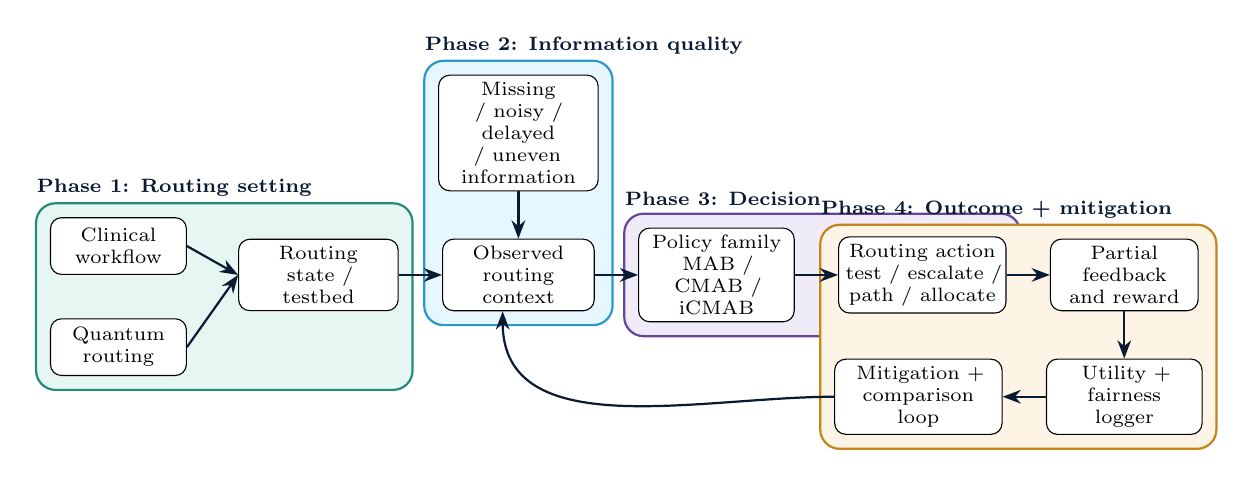
\begin{tikzpicture}[
font=\scriptsize,
box/.style={draw, rounded corners=4pt, align=center, text width=1.55cm, minimum height=0.72cm, inner sep=2.5pt, fill=white},
arr/.style={-Stealth, thick, draw=DeepNavy},
phase/.style={draw, rounded corners=7pt, inner sep=5pt, thick},
phaselabel/.style={font=\scriptsize\bfseries, text=DeepNavy, anchor=west}
]
\node[box] (clin) {Clinical\\workflow};
\node[box, below=0.55cm of clin] (quant) {Quantum\\routing};
\node[box, right=0.65cm of clin.south east, anchor=west, text width=1.85cm] (env) {Routing\\state /\\testbed};
\node[box, right=0.55cm of env, text width=1.75cm] (ctx) {Observed routing\\context};
\node[box, above=0.60cm of ctx, text width=1.85cm] (deg) {Missing / noisy /\\delayed / uneven\\information};
\node[box, right=0.55cm of ctx, text width=1.80cm] (pol) {Policy family\\MAB / CMAB / iCMAB};
\node[box, right=0.55cm of pol, text width=1.95cm] (act) {Routing action\\test / escalate /\\path / allocate};
\node[box, right=0.55cm of act, text width=1.70cm] (fb) {Partial feedback\\and reward};
\node[box, below=0.60cm of fb, text width=1.80cm] (log) {Utility + fairness\\logger};
\node[box, left=0.55cm of log, text width=1.95cm] (mit) {Mitigation +\\comparison loop};

\begin{scope}[on background layer]
\node[phase, fill=PhaseGreen!12, draw=PhaseGreen!80!black, fit=(clin)(quant)(env)] (p1) {};
\node[phase, fill=PhaseBlue!12, draw=PhaseBlue!80!black, fit=(ctx)(deg)] (p2) {};
\node[phase, fill=PhasePurple!12, draw=PhasePurple!80!black, fit=(pol)(act)] (p3) {};
\node[phase, fill=PhaseOrange!12, draw=PhaseOrange!80!black, fit=(fb)(log)(mit)] (p4) {};
\end{scope}

\node[phaselabel] at ([xshift=-0.10cm,yshift=0.18cm]p1.north west) {Phase 1: Routing setting};
\node[phaselabel] at ([xshift=-0.10cm,yshift=0.18cm]p2.north west) {Phase 2: Information quality};
\node[phaselabel] at ([xshift=-0.10cm,yshift=0.18cm]p3.north west) {Phase 3: Decision};
\node[phaselabel] at ([xshift=-0.10cm,yshift=0.18cm]p4.north west) {Phase 4: Outcome + mitigation};

\draw[arr] (clin.east) -- (env.west);
\draw[arr] (quant.east) -- (env.west);
\draw[arr] (env) -- (ctx);
\draw[arr] (deg) -- (ctx);
\draw[arr] (ctx) -- (pol);
\draw[arr] (pol) -- (act);
\draw[arr] (act) -- (fb);
\draw[arr] (fb) -- (log);
\draw[arr] (log) -- (mit);
\draw[arr] (mit.west) to[out=180,in=270] ([xshift=-0.20cm]ctx.south);
\end{tikzpicture}%
}
\caption{Color-coded shared domain model. The same four phases support both settings while preserving domain-specific meanings for routing state, action, reward, and fairness metrics.}
\label{fig:domain_model}
\end{figure*}

The domain model also explains how the components interact. The testbed produces a routing state, the observed context exposes only the information currently available, the degraded-context mechanism captures why some groups may receive weaker evidence, the policy selects a routing action, and the environment reveals only partial feedback for the chosen action. The logger then tracks both utility and fairness over time. These design choices relate directly to the diagram: the project studies fairness where the pipeline is most vulnerable, namely the transition from imperfect information to routing action.

\section{Why This Design}
This design was chosen for explicit reasons rather than convenience. First, the simulation-first clinical environment makes it possible to study diagnostic routing under controlled missingness, delay, noise, and subgroup-specific information loss without depending on sensitive patient records. Second, the quantum testbed builds on an existing routing and resource-allocation foundation, so the second branch is a technically credible environment rather than a toy example. Third, the shared framework is stronger than simpler alternatives. A single-domain study would not show whether the same fairness-aware routing logic survives across different systems. A contextual-only study would hide whether richer information truly improves disparity relative to lower-information baselines. A post-hoc audit would miss the core claim that fairness must be measured during learning under partial feedback.

This also answers why the approach should be done this way instead of following already familiar patterns. Prior work can be separated into valuable but incomplete pieces: clinical fairness studies are often offline or pipeline-specific, while routing studies often prioritize utility and robustness before fairness. The present design combines those strands into one fair online-routing comparison. That integration is the key advantage: the project can identify performance failures that are directly tied to unfair routing, test whether the same fairness logic transfers across both domains, and build toward future systems that treat fairness as part of routing quality rather than as an afterthought.

\section{Implementation Plan}
The implementation plan follows from the phased domain model. The clinical branch will simulate sequential routing through screening, confirmatory testing, and escalation. The quantum branch will integrate repeated path selection and entanglement/resource allocation under probabilistic links and changing conditions. Both environments will expose the same policy interface so that MAB, CMAB, and informative-context variants can be evaluated in one execution pipeline.

Reward design will capture domain-specific utility outcomes such as diagnostic accuracy, intervention cost, delivery success, and latency. Fairness design will capture disparities that matter inside each routing setting, including false-negative or delayed-escalation gaps in the clinical case and service-equity gaps in success or latency across flow groups in the quantum case. Per-step logging, fixed random seeds, explicit configuration files, and modular runs support reproducibility, while at least one fairness-aware mitigation mechanism will be evaluated inside the same framework. For that reason, the implementation is not a disconnected checklist; it is the operational consequence of the routing model shown in Figure~\ref{fig:domain_model}.

\begin{thebibliography}{9}\setlength{\itemsep}{0em}
\bibitem{garcia2025equitable_bioinformatics}
Garcia, P. Z. Equitable Bioinformatics: Enhancing Diagnostic Decision-Making through {RNA}
and Biomarker Data. Course paper (ISTE 780 Phase 4), Rochester Institute of Technology,
2025.
\bibitem{garcia2026threat_aware_quantum_routing}
Garcia, P. Z. Threat-Aware Evaluation of Quantum Entanglement Routing and Qubit Allocation
via Hybrid Contextual Bandits. Unpublished manuscript (GA-Work internal draft), Rochester
Institute of Technology, 2026.
\end{thebibliography}

\end{document}
